
In Appendix~\ref{appendix:exp6_items},
I plotted the time course analyses from Chapter 6
separately for each of the CRT problems.
The trends for problem 1, the so-called bat-and-ball problem
were slightly different from the other problems.
In particular, in Figure~\ref{fig:exp6-heuristic-to-chosen-by-item},
participants appear to be faster to move towards the heuristic response
on the no-conflict version of the bat-and-ball problem,
where this response is correct,
than on the conflict version, where it is incorrect,
as predicted by the conflict monitoring and intuitive logic theories.
However, averaging across all problems,
the reverse is true, as participants are generally slower to approach this response.

Mixed effects models, of the type used throughout this thesis,
provide a means of formally analysing differences between problems,
as regression weights can be allowed to vary for each problem.
However, due to the complexity of the model already used,
it was not possible to include such random slopes
for the time course data shown in Figure~\ref{fig:exp6-heuristic-to-chosen-by-item}.
Fortunately, the same effect is captured
by the analysis of participants' response times, reported in Chapter 6.

Therefore, I fit a model were log-transformed response times
for heuristic responses to no-conflict problems
were compared to those for heuristic responses to conflict problems.
I included random intercepts for each participant and each problem,
and crucially, random slopes for each problem,
meaning the effect of interest was allowed to vary between problems.
As was the case in the model reported in Chapter 6,
there was no significant difference between the conditions overall,
but participants were in general \emph{faster} on conflict problems,
contrary to the predictions of the conflict monitoring theory
($e^{\beta}$ = 96\%, CI = [83\%, 110\%], t(7.3) = 0.551, p > .5).

The estimated effects of condition for each problem
are shown in Table~\ref{tab:exp6-appendix-table},
and in Figure~\ref{fig:exp6-appendix-figure}.
These show that participants were indeed slower
on the conflict version of the bat-and-ball problem,
as predicted by the conflict monitoring and intuitive logic theories.
However, the opposite was true for a number of other problems,
where participants were actually faster to respond
on conflict versions.
Therefore, the bat-and-ball problem
can be seen as an outlier in this sense.

\begin{table}[h]
  \centering
  \caption[]{
    Variation between problems in
    fitted mean response times for
    heuristic responses to no-conflict problems,
    and the change in response times
    for heuristic responses to conflict versions of the same problem.
    Changes greater than 100\% reflect
    slower responses on conflict problems,
    as predicted by the conflict monitoring
    and intuitive logic theories.
    95\% confidence intervals are also shown.
    \label{tab:exp6-appendix-table}
  }
  \begin{tabular}{lrrrr}
    \toprule
    Problem           & No-conflict RT (Seconds) & Change& Lower  & Upper\\
    \midrule
    1. Bat-and-ball   & 13.3           & 114.0\%               & 99.9\% & 130.2\%\\
    2. Widgets        & 18.8           & 105.6\%               & 92.5\% & 120.5\%\\
    3. Lily pad       & 30.3           & 75.8\%                & 66.4\% & 86.5\%\\
    4. Coin           & 12.8           & 92.1\%                & 80.7\% & 105.1\%\\
    5. Elves          & 23.5           & 89.7\%                & 78.6\% & 102.4\%\\
    6. Running track  & 20.6           & 99.6\%                & 87.2\% & 113.7\%\\
    7. Grades         & 15.2           & 106.3\%               & 93.1\% & 121.4\%\\
    8. Athletics team & 27.3           & 93.5\%                & 81.9\% & 106.8\%\\
    \bottomrule
  \end{tabular}
\end{table}

\begin{figure}[h]
  \centering
  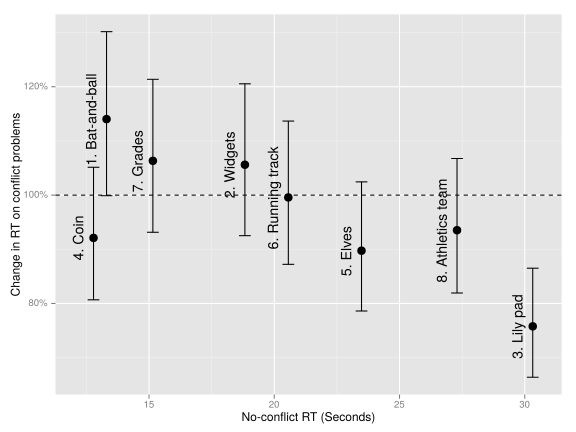
\includegraphics[width=.5\textwidth]{imgs/exp6/random_effects_rt.pdf}
  \caption[]{
    Variation between problems in
    fitted mean response times for
    heuristic responses to no-conflict problems,
    and the change in response times
    for heuristic responses to conflict versions of the same problem.
    Changes greater than 100\% reflect
    slower responses on conflict problems,
    as predicted by the conflict monitoring
    and intuitive logic theories.
    Error bars show 95\% confidence intervals.    
    \label{fig:exp6-appendix-figure}
  }
\end{figure}
